\documentclass{sigchi}

    % Use this section to set the ACM copyright statement (e.g. for
    % preprints).  Consult the conference website for the camera-ready
    % copyright statement.
    
    % Copyright
    \CopyrightYear{2016}
    %\setcopyright{acmcopyright}
    \setcopyright{acmlicensed}
    %\setcopyright{rightsretained}
    %\setcopyright{usgov}
    %\setcopyright{usgovmixed}
    %\setcopyright{cagov}
    %\setcopyright{cagovmixed}
    % DOI
    \doi{http://dx.doi.org/10.475/123_4}
    % ISBN
    \isbn{123-4567-24-567/08/06}
    %Conference
    \conferenceinfo{CHI'16,}{May 07--12, 2016, San Jose, CA, USA}
    %Price
    \acmPrice{\$15.00}
    
    % Use this command to override the default ACM copyright statement
    % (e.g. for preprints).  Consult the conference website for the
    % camera-ready copyright statement.
    
    %% HOW TO OVERRIDE THE DEFAULT COPYRIGHT STRIP --
    %% Please note you need to make sure the copy for your specific
    %% license is used here!
    % \toappear{
    % Permission to make digital or hard copies of all or part of this work
    % for personal or classroom use is granted without fee provided that
    % copies are not made or distributed for profit or commercial advantage
    % and that copies bear this notice and the full citation on the first
    % page. Copyrights for components of this work owned by others than ACM
    % must be honored. Abstracting with credit is permitted. To copy
    % otherwise, or republish, to post on servers or to redistribute to
    % lists, requires prior specific permission and/or a fee. Request
    % permissions from \href{mailto:Permissions@acm.org}{Permissions@acm.org}. \\
    % \emph{CHI '16},  May 07--12, 2016, San Jose, CA, USA \\
    % ACM xxx-x-xxxx-xxxx-x/xx/xx\ldots \$15.00 \\
    % DOI: \url{http://dx.doi.org/xx.xxxx/xxxxxxx.xxxxxxx}
    % }
    
    % Arabic page numbers for submission.  Remove this line to eliminate
    % page numbers for the camera ready copy
    % \pagenumbering{arabic}
    
    % Load basic packages
    \usepackage{balance}       % to better equalize the last page
    \usepackage{graphics}      % for EPS, load graphicx instead 
    \usepackage[T1]{fontenc}   % for umlauts and other diaeresis
    \usepackage{txfonts}
    \usepackage{mathptmx}
    \usepackage[pdflang={en-US},pdftex]{hyperref}
    \usepackage{color}
    \usepackage{booktabs}
    \usepackage{textcomp}
    
    % Some optional stuff you might like/need.
    \usepackage{microtype}        % Improved Tracking and Kerning
    % \usepackage[all]{hypcap}    % Fixes bug in hyperref caption linking
    \usepackage{ccicons}          % Cite your images correctly!
    % \usepackage[utf8]{inputenc} % for a UTF8 editor only
    
    % If you want to use todo notes, marginpars etc. during creation of
    % your draft document, you have to enable the "chi_draft" option for
    % the document class. To do this, change the very first line to:
    % "\documentclass[chi_draft]{sigchi}". You can then place todo notes
    % by using the "\todo{...}"  command. Make sure to disable the draft
    % option again before submitting your final document.
    \usepackage{todonotes}
    
    % Paper metadata (use plain text, for PDF inclusion and later
    % re-using, if desired).  Use \emtpyauthor when submitting for review
    % so you remain anonymous.
    \def\plaintitle{SIGCHI Animal Interface Framework}
    \def\plainauthor{Jacob Logas, Will Mitchell, Monira Khan, Lorita Freeman}
    \def\emptyauthor{}
    \def\plainkeywords{touchscreen; dog; framework; user interface; animal-computer interaction; required.}
    \def\plaingeneralterms{Documentation, Standardization}

    % llt: Define a global style for URLs, rather that the default one
    \makeatletter
    \def\url@leostyle{%
      \@ifundefined{selectfont}{
        \def\UrlFont{\sf}
      }{
        \def\UrlFont{\small\bf\ttfamily}
      }}
    \makeatother
    \urlstyle{leo}
    
    % To make various LaTeX processors do the right thing with page size.
    \def\pprw{8.5in}
    \def\pprh{11in}
    \special{papersize=\pprw,\pprh}
    \setlength{\paperwidth}{\pprw}
    \setlength{\paperheight}{\pprh}
    \setlength{\pdfpagewidth}{\pprw}
    \setlength{\pdfpageheight}{\pprh}
    
    % Make sure hyperref comes last of your loaded packages, to give it a
    % fighting chance of not being over-written, since its job is to
    % redefine many LaTeX commands.
    \definecolor{linkColor}{RGB}{6,125,233}
    \hypersetup{%
      pdftitle={\plaintitle},
    % Use \plainauthor for final version.
    %  pdfauthor={\plainauthor},
      pdfauthor={\emptyauthor},
      pdfkeywords={\plainkeywords},
      pdfdisplaydoctitle=true, % For Accessibility
      bookmarksnumbered,
      pdfstartview={FitH},
      colorlinks,
      citecolor=black,
      filecolor=black,
      linkcolor=black,
      urlcolor=linkColor,
      breaklinks=true,
      hypertexnames=false
    }
    
    % create a shortcut to typeset table headings
    % \newcommand\tabhead[1]{\small\textbf{#1}}


% End of preamble. Here it comes the document.
\begin{document}

    \title{\plaintitle}

    \numberofauthors{4}
    \author{%
    \alignauthor{Jacob Logas\\
        \affaddr{Georgia Institute of Technology}\\
        \affaddr{Atlanta, GA 30332, USA}\\
        \email{logasja@gatech.edu}}\\
    \alignauthor{Will Mitchell\\
        \affaddr{Georgia Institute of Technology}\\
        \affaddr{Atlanta, GA 30332, USA}\\
        \email{wmitchell30@gatech.edu}}\\
    \alignauthor{Monira Khan\\
        \affaddr{Georgia Institute of Technology}\\
        \affaddr{Atlanta, GA 30332, USA}\\
        \email{monirakhan@gatech.edu}}\\
    \alignauthor{Lorita Freeman\\
        \affaddr{Georgia Institute of Technology}\\
        \affaddr{Atlanta, GA 30332, USA}\\
        \email{lorita.freeman@gatech.edu}}\\
    }

    \maketitle

    \begin{abstract}
        In the past, touchscreen interfaces created for dogs have made liberal use of buttons and avoided other user interfaces common in human applications. Here, we present a framework on which interfaces can be developed and tested. The framework obtains with metrics such as touch position over time and time to complete. To demonstrate the framework’s efficacy, we build a simple slider interface with various variable attributes that we will then use to study how a dog interacts with a slider. Our hope is this framework can be used to quantifiably evaluate interfaces created for animals.
    \end{abstract}

    \category{H.5.m.}{Information Interfaces and Presentation
    (e.g. HCI)}{Miscellaneous} \category{See
    \url{http://acm.org/about/class/1998/} for the full list of ACM
    classifiers. This section is required.}{}{}

    \keywords{\plainkeywords}

    \section{Introduction}
        Touchscreens are ubiquitous in our daily lives, from our phones to our watches we have made great use of touchscreen displays to explore many use cases. Good touchscreen interactions are the focus of much HCI research because of its ubiquity. As with most other forms of technology though, interfaces have been developed with a human audience in mind. However, dogs are frequently able to take many complex tasks upon themselves and have demonstrated ability to interact with touchscreen displays among other technologies \cite{Zeagler2016,Zeagler2014,Wallis2017,Aust2008,Zeagler2016a,Byrne2014}. With the rising field of ACI, more and more interfaces will be designed for animals on touchscreen devices however there is little information on which interfaces are transferable between species and ways to evaluate interfaces. This severely limits a designer’s ability to design a truly user-centered application.
    
    \section{Background and Related Work}
    \subsection{Animal Cognition}
        Animal cognition research until recently believed dogs to be too changed by their domestication to have any interesting cognitive ability worthy of study. Recently though, the perception of dog cognition has significantly improved such that most animal cognitive studies make use of them. Obtaining subjects is relatively easy as much of the population have companion dogs and cognitive studies have low risk of injury. Additionally, all one needs to run a dog study is an empty room \cite{Morell2009}.
        
        Studies into domestic dog cognition has provided evidence of dogs’ ability to reason. Aust et al. investigates inferential reasoning in dogs by providing dogs a set of suboptimal stimuli known to the dog and one unknown stimuli. If the dog chooses the unknown stimuli, it gives evidence of reasoning by the dog that if the optimal stimuli is not among the known, it must be the unknown.This is accomplished through use of a touchscreen with icons which, in addition to giving evidence of inferential reasoning, is evidence of dogs’ ability to reason meaning behind icons in a digital interface \cite{Aust2008}.
        
        Range et al. added to this evident ability of dogs by studying dogs’ ability to categorize images based on content. The study uses a touchscreen on which dogs are shown images with either only landscapes or only dogs which are categorized by the subjects with high accuracy. To ensure no bias to the specific dog images, a photo editing tool is used to extract the dogs in the images and post them over the landscape images. This led to a decrease in accuracy however categorization was well above random chance \cite{Range2008}.
        
        Cognitive science may give an indication of dogs’ abilities to use existing technology, but one must consider not only if an animal can use an interface but also if the interface improves its livelihood. This is what led to the rise of Human-Computer Interaction (HCI) as a discipline within computer science and now the extension to Animal-Computer Interaction (ACI).

    \subsection{Animal-Computer Interaction}
        Technology has long been the new evolutionary force for humankind, allowing us to no longer need to adapt to our environment but create environments amicable to us. Companion animals have enjoyed some of the comforts afforded to us tangentially such as air conditioning, clean water, and complex medical procedures. However, much of user-centered technology has been solely developed for humans. One may argue that this is because animals lack the skill to make use of these tools, to which one can point to studies that find animals to make tools and even exploit human tools for their ends \cite{Hunt2004}.
        
        This is not to say there have been no technologies developed for use by animals, however they are often to enhance the human’s relationship with the animal. These include automatic milkers, GPS collar trackers, and interfaces used for behavioral experiments \cite{Epstein2000,Garton2001}. In addition, service animals have been trained to take on tasks that are difficult for their handlers to perform such as operating light switches or washing machines \cite{Mancini2017a}. Consumer devices ostensibly made for companion animals have also come to the market in the form of tracking collars or teleconferencing systems with the promise of improving the animal’s life.
        
        Though in all of these technologies, the animals have no interaction with the development process. Humans are making the devices in the way that best serves their needs with only some consideration given to the animal using it. Questions from HCI are therefore ignored when applied to animals. Instead of questioning how the interaction would influence the animal’s capabilities, activities, and experience we think in terms of how it will affect the livelihood of the owner with relation to the animal.
        
        This has changed with the rise of ACI where the concern of how the animal is experiencing the technology is considered. As many researchers from the field of HCI were the ones to pioneer this field, they brought their core considerations with them. User experience is of high importance in HCI and that has transferred over to ACI as was user-centered and participatory design \cite{Forlizzi2004,10.1007/978-3-642-15231-3_11,Muller1993}. Unfortunately, many of these considerations prove to be more difficult when there is no way to reliably obtain the participant’s experience objectively.
        
        In the face of fragmentation of the field, Mancini called for the development of ACI as a discipline with three core aims. First, studying and theorising animal interaction with technology in a naturalistic setting. Second, develop user-centered technology to improve welfare, support their activities, and foster interspecies relationship. Finally, allow animals to be stakeholders in the design of technology by focusing on them as the main user.
        
        One major obstacle in developing with animals as opposed to for animals is that humans are making the interfaces. Therefore, there is a disassociation between the proponents and intended beneficiaries. It is arguable that the interests of humans and other animals are not always aligned and often are in direct competition and that human interpretation of animal interests are significantly biased with the human’s experiences and world views. Some posit that animals’ are unable to communicate in a way that contributes to the design of an interface or that the inability to simply relate complex ideas and opinions results in a disparity of power between the designer and animals. Lawson et al. argues that this leads to technology that is explotative of animals \cite{Lawson:2015:PUT:2702123.2702260}.
        
        To overcome these obstacles, several frameworks have been proposed to conceptualise the animal interaction with technology and their involvement in the design process. Resner extended traditional design concepts to develop a remote dog training system \cite{Resner2001}. Paci et al. and Mancini et al. reviewed interaction design principles to improve animal biotelemetry wearability and accessibility of canine interfaces \cite{Paci2016, Mancini:2011:AIM:1978822.1978836}.

    \subsection{Animal Interfaces}
        A major focus of recent studies in ACI have been the use of computer devices for improving communication between working dogs and their handlers. We will briefly touch on some of the more relevant cases.
        
        Byrne et al. introduced an interface that is mounted on the dog’s harness which vibrates on either side. This study found that dogs are able to be taught to discriminate between the vibrations and react with some action when prompted by the motors. This study not only introduced a usable interface but also gave insight into some unexpected considerations that need to take place when developing and testing interfaces. This is especially true of dogs who are able to quickly learn triggers, even if subconsciously expressed \cite{Byrne2014}.
        
        Zeagler et al. presented another wearable device that is mounted on the dog’s harness. This device has a capacitive sensor on either side that the dog can touch with its nose for communication purposes. Through subsequent trials, it was found that the sensor could be accidentally activated by a dog’s ear or surrounding environment. This was an interesting finding as it gives more information to more considerations that need to be taken when working with dog physiology \cite{Zeagler2016a}.
        
        Most relevant to this work however, is the work done by Zeagler et al. on an emergency alert system that is operated by a service dog when at home. The authors identified several pitfalls when designing a digital interface for dogs. First, that a capacitive touchscreen after some use will become non-responsive because of accumulated slobber. To fix this, an infrared-based touchscreen is advised. Additionally, it was discovered that a constantly emitting display such as an LED monitor is preferable to say a projector which, because of its method of color emittance, caused the dogs to lose the button positions. Finally, the authors find that larger buttons are preferable as the dog is interacting with its nose and therefore does not have a full view of the screen \cite{Zeagler2014}.

    \section{Metrics}
        As animals are unable to provide responses to a provided interface in the traditional sense, metrics must be studied to gain insight into an interface’s efficacy. Here we measure the velocity of the interaction, the tapping pressure, accuracy of touch, and force exerted in a direction. In addition to these we will be measuring how long the interface takes for an animal to use and the path that the animal’s interaction takes if it is a draggable interface as the slider is. We believe these metrics are key in determining a dog’s feeling about an interface, especially when used in concert with a physical observation of the task being done.

    \section{Slider Interface}
        Multiple variations of a slider were designed for the interface to test different aspects of a dog’s ability to understand interfaces. The first interface design is simple, it is a horizontal slider with differently shaped handles, some with directionality to them and others that have missing parts. It is important to note that in all these interfaces, the parts can be swapped so that colors, shapes, tracks, etc. can be modified independently. The interfaces are designed to be fully rotatable and scalable as well to create even more variations for testing.

        Another variation of the slider that is drafted below changes colors in the interface as the dog moves the handle along the track. One changes the color of the handle only and could give insight into how much the dog pays attention to the color cues when interacting or if the color can actually be perceived when so close to the display. Another transitions the colors as the slider is being moved, allowing the dog to see the color change more clearly.

        Audio cues are thought to be important to dogs when they cannot visually obtain an idea of progression. Additionally, audio cues are very important to training and choosing the correct audio could positively impact their reward when correctly using the interface. To this end, several audio cues have been explored. A rising or lowering pitch as the slider moves is a possible cue as is one that increases at certain thresholds. Overall, audio cues are important to the experience of the interface and more options are being explored.

        Adding a physicality to the slider is another interesting interaction that we believe will improve the interface for a dog. By giving the handle physical attributes like rolling downward when released on a slant, we believe the dog will become more engaged with the interface. Additionally, this interaction could be useful for training easily distracted dogs to use the touchscreen.

        The most difficult interface we designed represent cognitively difficult tasks for the dogs. One of the sliders would have a dip in the middle, and another might be U or S shaped, to make the trail more difficult for the dog to follow. Another would be a slider that would rotate as it was moved, to make it harder to move in a straight line. This would be something similar to what would be required of using a website, for example.
    
    \section{Future Work}
        Our future work from here on lies entirely in the implementation of the plans we set out in the previous section. Obviously a large part of this is going to be in the coding of these to work as actually described. We believe that we can at the very least get the multiple shape and color ones working correctly, using multiple different sounds. We are also in the process of trying to find dogs that we can test with to see if our prototypes perform as expected. This will probably require creating interfaces that work for outputting testing data as well instead of simply going for a proof of concept.
    
    \section{Conclusion}
        Research based on dogs, technology, and touchscreens has been in the works for a long time. With this project, we wanted to expand on the current research by creating a variety of interfaces to see how dogs react and interact with them. Testing the dogs’ capabilities with different interfaces will show us what adjustments and improvements we can make to these interfaces. This opens up the possibilities of what dogs will be able to do with technology in the future. Service dogs, police dogs, and even our pets can already aid us in so many ways, and with the progression of this research our companions will be able to take on greater roles in our lives and in our society.

    \bibliography{midterm}
    \bibliographystyle{SIGCHI-Reference-Format}

    \clearpage

    \appendix
        \begin{figure}[h]
            \centering
            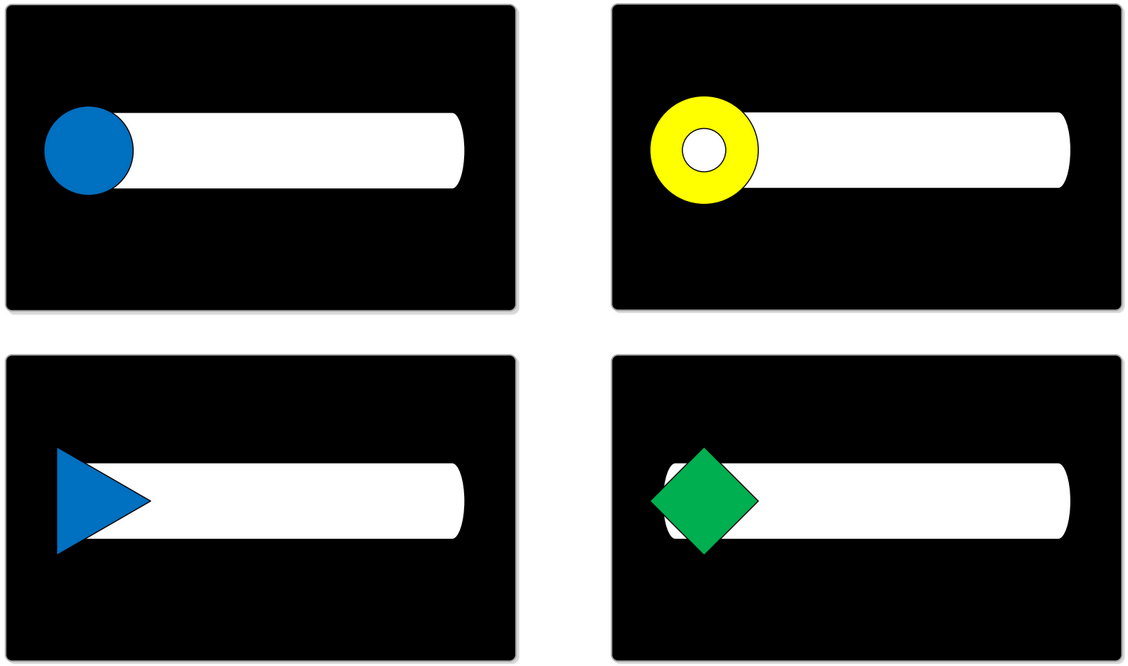
\includegraphics[width=\textwidth/2]{figures/slider_shapes.png}
            \caption{Different shapes and colors for the slider handle (kept in dog's visible color spectrum).}
            \label{fig:mockup1}
        \end{figure}
        \begin{figure}[h]
            \centering
            
\includegraphics[width=\textwidth/4]{figures/curved-slider.png}
            \caption{A mockup of a challenging slider.}
            \label{fig:mockup2}
        \end{figure}
        \begin{figure}[b]
            \centering
            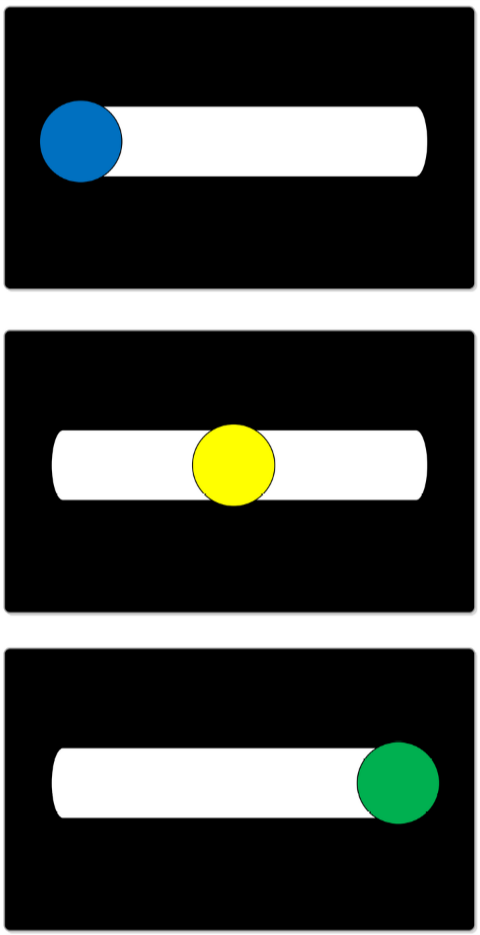
\includegraphics[height=\textheight/2]{figures/handle_change.png}
            \caption{Changing color handle as slid from beginning to end.}
            \label{fig:mockup3}
        \end{figure}
        \begin{figure}[h]
            \centering
            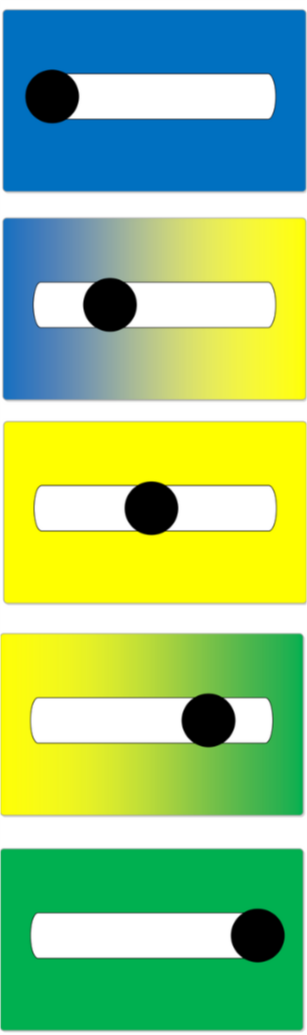
\includegraphics[height=\textheight]{figures/background-transition.png}
            \caption{Illustration of how a background transition could occur.}
            \label{fig:mockup4}
        \end{figure}

\end{document}